\documentclass[conference]{IEEEtran}
%\documentclass[9pt]{acmieeeSC}
%\documentclass[9pt]{acmsiggraph}      % review
%\documentclass{acmsiggraph}      % review
%\documentclass[widereview]{acmsiggraph}  % wide-spaced review
%\documentclass[preprint]{acmsiggraph}    % preprint

%% Uncomment one of the four lines above depending on where your paper is
%% in the conference process. ``review'' and ``widereview'' are for review
%% submission, ``preprint'' is for pre-publication, and ``final'' is for
%% the version to be printed.

%% These two line bring in essential packages: ``mathptmx'' for Type 1 
%% typefaces, and ``graphicx'' for inclusion of EPS figures.

\usepackage{mathptmx}
\usepackage{graphicx}
%\usepackage{psfig}
\usepackage{algorithmic}
\usepackage{algorithm}

\usepackage{subfigure}% for multiple figures in one big figure env

%% use this for zero \parindent and non-zero \parskip, intelligently.

\usepackage{parskip}
\usepackage{cite}

%% If you are submitting a paper to the annual conference, please replace 
%% the value ``0'' below with your OnlineID. If you are not submitting this
%% paper to the annual conference, you may safely leave it at ``0'' -- it 
%% will not be included in the output.

%% need to document this!

%\acmformat{print}

%% Paper title.

\begin{document}

\title{
UniDQP: Making MapReduce Scheduling Decisions with an Awareness of the Cached Data Location 
\thanks{This research was supported by UNIST Supercomputing Center and 
the National Research Foundation of Korea(NRF) 
funded by the Ministry of Education, Science and Technology (2011-001475)}
}

%% Author and Affiliation (multiple authors).
%\author{\IEEEauthorblockN{Deukyeon Hwang, Jaewon Kwak, Wok-Ki Jeong, Beomseok Nam}
%        \IEEEauthorblockA{ School of Electrical andComputer Engineering\\
\author{{Vicente Bolea Sanchez and Beomseok Nam} \\
        School of Electrical andComputer Engineering\\
        Ulsan National Institute of Science and Technology  \\
        Ulsan, Korea, 689-798 \\
        Email: vicente.bolea@gmail.com, bsnam@unist.ac.kr
}


%%%%%% START OF THE PAPER %%%%%%


%% The ``\maketitle'' command must be the first command after the
%% ``\begin{document}'' command. It prepares and prints the title block.

\maketitle

%% Abstract section.


\begin{abstract}

%In modern query processing systems, the caching facilities are distributed and
%scale in accordance with the number of servers. To maximize the overall system
%throughput, the distributed system should balance the query loads among
%servers \emph{and} also leverage cached results.  In particular, leveraging
%distributed cached data is becoming more important as many systems are being
%built by connecting many small heterogeneous machines rather than relying on a
%few high-performance workstations.  
%
%Although many query scheduling policies exist such as round-robin and
%load-monitoring, they are not sophisticated enough to both balance the load
%and leverage cached results.  
%

In this work, we present a novel distributed file processing framework called
\emph{UniDQP} that takes into account the dynamic nature of file I/O request 
distribution and remote contents of distributed caching infrastructure.  The
job scheduler of the framework makes scheduling decisions based on the 
spacial location of the queries. 
In addiction, we propose an innovate scheme enhancing the cohesion of system.
%I dont know how to describe the above sentence

%two layer back-end
%servers structure achieving a high cohesion with the scheduler.

\end{abstract}

\section{Introduction}

Distributed and parallel query processing middleware systems have been used for
decades to solve large and complicated scientific problems as substantial
performance gains can be achieved by exploiting data and computation
parallelism.  MapReduce framework has recently gained tremendous popularity as
a key distributed and parallel query processing framework due to its
scalability and easy programming model~\cite{}. However, MapReduce framework is
not designed to leverage the large amount of memory space available in the
back-end distributed servers since its target applications are mostly
performing one time data analysis.  Unlike the web data processing applications
scientific datasets are often reused by multiple jobs and semantic caching
plays an important role in improving the system throughput and job response
time.  Another design decision that we have to make concerens is the data skew
challenge in MapReduce framework. In~\cite{IBRAHIM10, KWON10, LIN09} it has
been reported that some map tasks (stragglers) take significantly longer than
the average execution time of other map tasks. In order to mitigate the
stragglers problem, MapReduce framework runs some backup tasks to alleviate the
problem, however the back-up tasks do not help when the input datasets are not
well balanced. 
  
In this work, we present a distributed and parallel query processing middleware
framework - {\em Orthrus} which takes into account the large memory space in
back-end servers and makes scheduling decisions based on the cached data
objects in the memory instead of data file location. Orthrus is a two layer
architecture as it deploys a layer of distributed semantic caches on top of a
distributed file system layer. In order to balance the system load and to
improve data reuse rate, the front-end scheduler of Orthrus needs to estimate
the cached contents in distributed semantic cache layer for data reuse, and
assign equal amout of jobs to each server for load balancing.  A challenge in
estimating the remote cache contents in distributed query processing framework
is that the front-end scheduler should exchange large amount of information
about remote caches as the cached objects in each server change very fast as
they process jobs. Capturing a global snapshot of remote servers' cache
contents is certainly a very expensive operation especially in a large scale
system. Another challenge in designing cache-aware query scheduling policies is
that the scheduling algorithm must be light-weight so that it doesn't
bottleneck the front-end scheduler. 

In this poster presentation, we present the two layer architecture of
our distributed and parallel query processing framework, its scheduling
algorithms, data migration policies, and preliminary results of performance 
evaluation.


\section{Orthrus: Distributed Query Processing Framework}


\begin{figure}
\centering 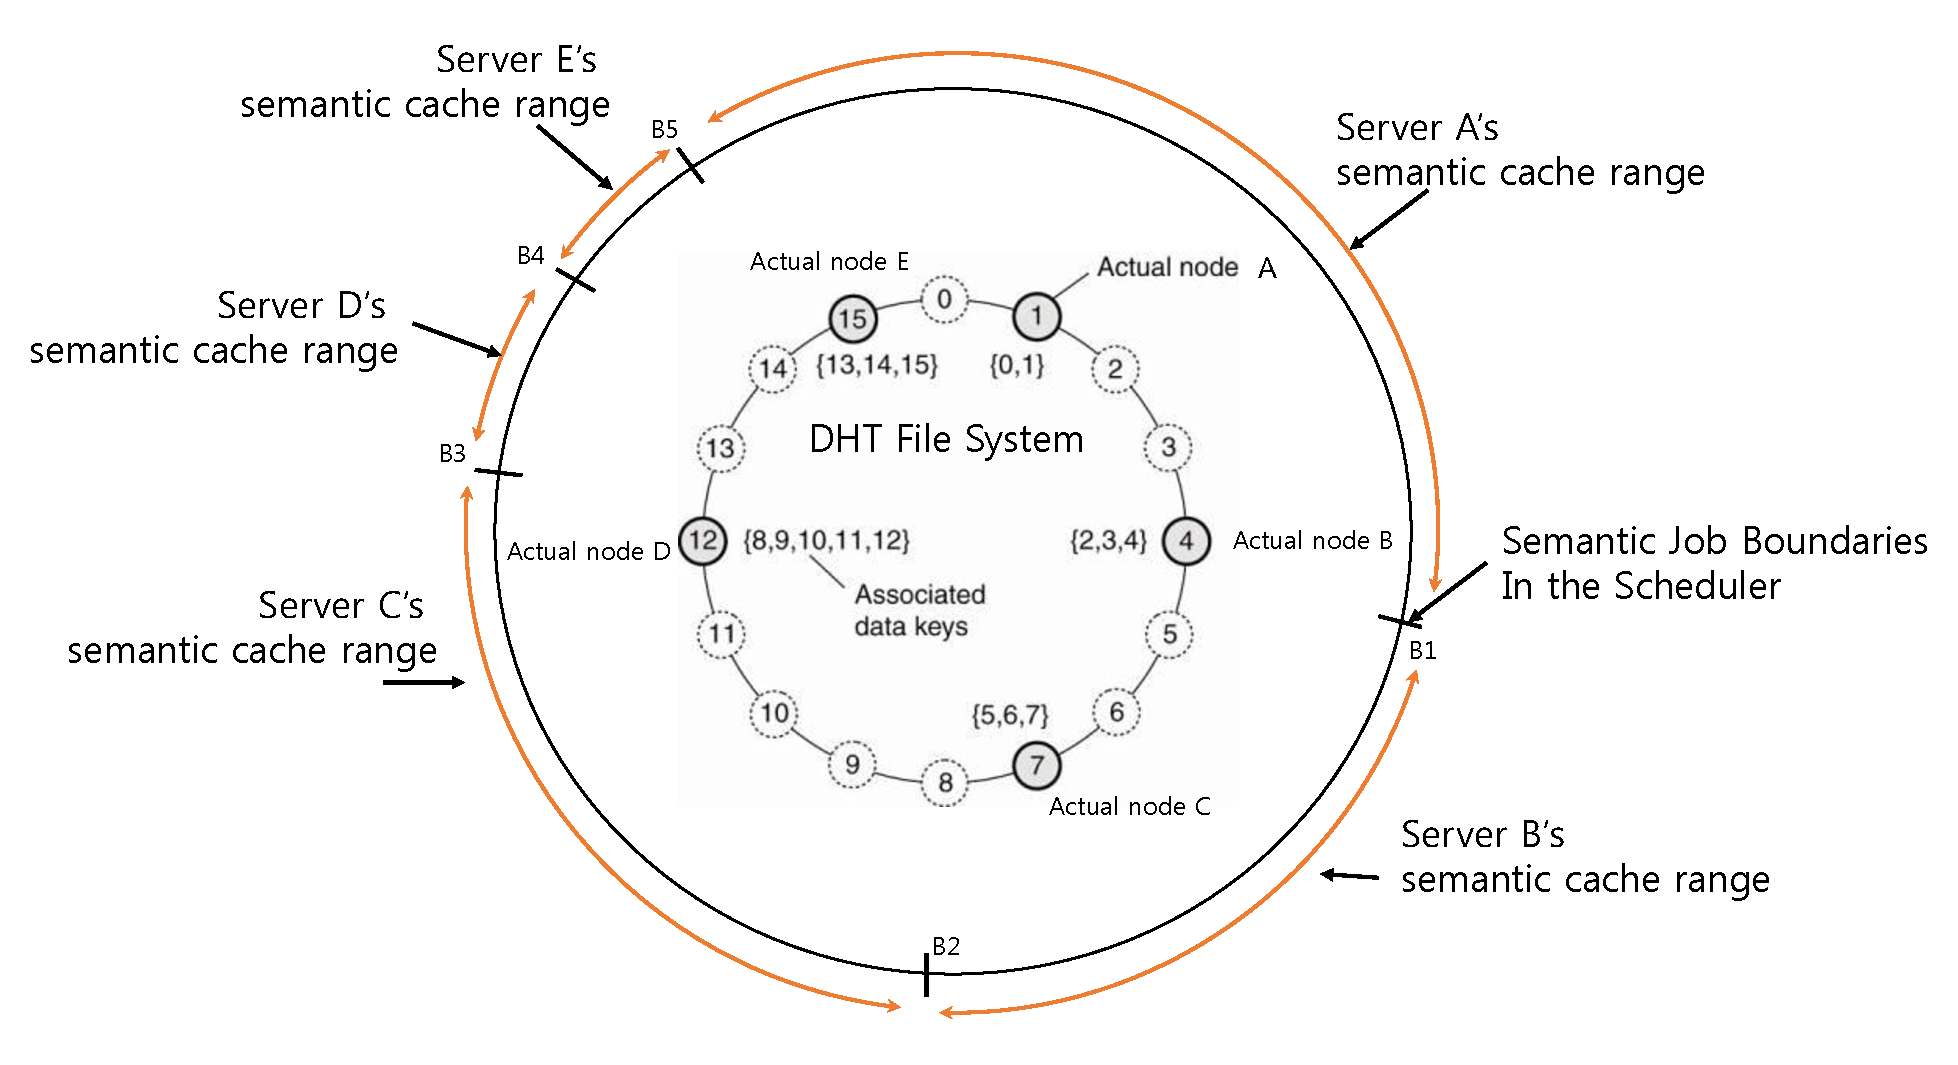
\includegraphics[width=.48\textwidth]{arch.eps}
\caption{\textit{Two layers structure of back-end servers.}}
\label{fig:fig1}
\end{figure}

%Previous policies
%Starting on the basis that in a tipical use of a DQP, the probability of an 
%access near located data that the previous access. 

%Our middle-ware makes some assumsions. Firstly considering an hard-disk
%as a bottle-neck and providing a much faster network.


We propose a framework composed of a set of accesible front-end servers 
and a collection of back-end caching servers organized in a two layers peer-to-peer structure.
%UniDQP can be seen as a two layers hybrid peer-to-peer system with scheduler.


%one outer layer which reflects the cached dataset,
%and one inner layer which represent the full dataset dispersed among the existing
%hard-disks.

%the where while the every 
%back-end server has a fixed section of the data store in its hard-disk, every data cached
%in the system is accessible from every back-end node.
%The most important property of this layer is that

\subsubsection{Inner layer}
It consists in a set of not mutable static segments which represents the range of the dataset corresponding
to each back-end server. This layer is visible from every back-end servers through its hashing lookup table.

\subsubsection{Outer layer}
Analogously, we propose a non-static layer divided in mutable boundaries which 
represents the current status of the cached data. This layer is not completely visible, where
in contrast to the inner layer, each back-end node only knows its boundary and neighbors.
Those boundaries are in a continuous movement due to our spacial algorithm.

%is not static and its continuously changing, also a back-end
%server only knows about its own boundaries.

%\subsection{Hashing lookup table}
%In order to locate the correct back-end server. We propose an share and distributed 
%lookup table which store for each data the server where it belongs.
%
%\subsection{Pop policy}
%One of the most important functionability in systems with large dataset is the
%discarding policy, since a backend node only can cache a small percentage of its dataset.
%UniDQP will simply discard those nodes whichthe least-recently-used or less likely to be accessed
%data to its closer neighbor backend server.
%has an lookup table which 

\subsection{Data migration}
An intensive use of data migration is necessary to guarantee a high cohesion between the 
front-end and back-end servers. Our framework accomplish two main problems making use of this policy:

\subsubsection{Overlap of the boundaries}
Due to a continous movement of the boundaries of the outer layer, at some point the data located near by
its boundary could be out of its original range, for this reason our framework corrects the overlap migrating
overlapped data to the range where it belongs.

\subsubsection{Requesting data}
As the ranges are continously moving, the scheduler can not know accurately which back-end node contains
the requested data. In order to overcome this problems our framework provide a hashing lookup table
to each back-end server indicating which range in the inner layer contains the requested data. 
In case of failure of the scheduler, the requested data will be readed from the corresponing back-end server
and cached in the back-end server selected by the scheduler.

%where whenever a query arrives in a given back-end server,
%in case that such back-end server does not contain that data, it consults its lookup table and redirects
%the query to the back-end node whose has assign the range of dataset in the inner layer which contains
%that query. Also, this migration process is use to balance the system.


%On the other hand, our framework needs a scheduler to redirect the queries and compute the boundaries.

\begin{figure}
\centering 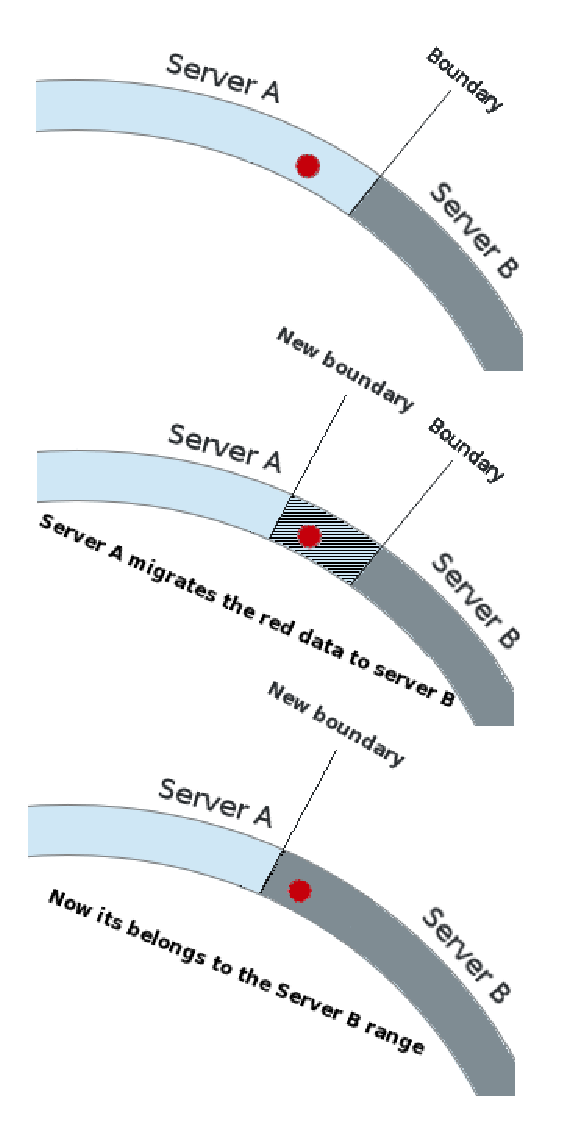
\includegraphics[width=.20\textwidth]{graphic1.eps}
\caption{\textit{Two layers structure of back-end servers.}}
\label{fig:fig2}
\end{figure}

%Our middle-ware performance is based on the data migration between the back-end servers.
%In several cases it will migrate data. Firstly, whenever the cache is full it will migrate
%at first the farthest element from the EMA point in the cache the least-recently-accessed data


%actual policy

%\begin{figure*}[!ht]
%\centering
%\subfigure[Query Response Time]{
%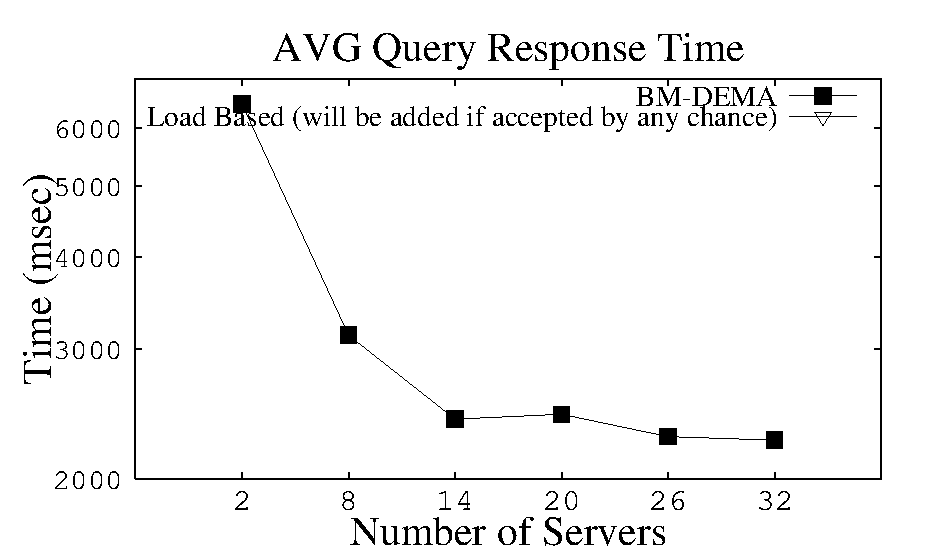
\includegraphics[width=.38\textwidth]{nservers.qwet.eps}
%\label{fig:real-qwet}
%}
%\subfigure[Hit Ratio]{
%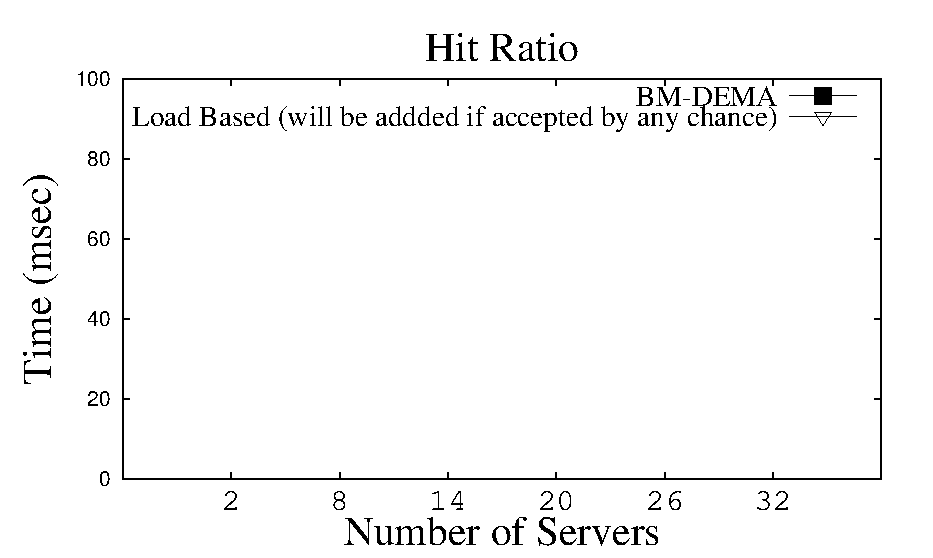
\includegraphics[width=.38\textwidth]{nservers.hit.eps}
%\label{fig:real-balance}
%}
%\caption{\textit{Query Response Time and Hit Ratio with Varying \# of Back-end Servers}}
%\label{fig:nservers}
%\end{figure*}



\section{Experiments}



\section{Conclusion} \label{conclusion-section}



%\nocite{*} 
% This causes all the item in bib file to be included in the reference - BSNAM
%\bibliographystyle{acmsiggraph}

\bibliographystyle{IEEEtran}
\bibliography{/home/bsnam/doc/bib/bsnam.bib}

\end{document}
